\usetikzlibrary{calc,arrows.meta,patterns,angles,quotes}
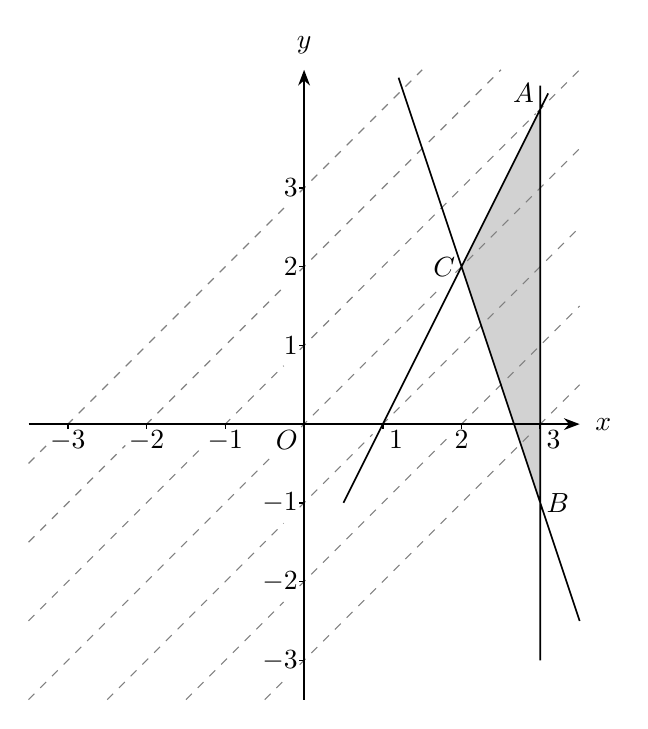
\begin{tikzpicture}[x=1cm,y=1cm,line width=.6pt,font=\normalsize,>=Stealth]
\coordinate (A) at (3.0000000000,4.0000000000);
\coordinate (B) at (3.0000000000,-1.0000000000);
\coordinate (C) at (2.0000000000,2.0000000000);
\fill[gray!35] (A)--(B)--(C)--cycle;

\draw[gray,dashed,line width=.4pt] (-0.5000000000,-3.5000000000)--(-0.2565943061,-3.2565943061);
\draw[gray,dashed,line width=.4pt] (-0.0558121702,-3.0558121702)--(2.8696554354,-0.1303445646);
\draw[gray,dashed,line width=.4pt] (2.9888744058,-0.0111255942)--(3.5000000000,0.5000000000);
\draw[gray,dashed,line width=.4pt] (-1.5000000000,-3.5000000000)--(-0.2595384555,-2.2595384555);
\draw[gray,dashed,line width=.4pt] (-0.0570470217,-2.0570470217)--(1.8690016132,-0.1309983868);
\draw[gray,dashed,line width=.4pt] (1.9888744058,-0.0111255942)--(3.5000000000,1.5000000000);
\draw[gray,dashed,line width=.4pt] (-2.5000000000,-3.5000000000)--(-0.2595187463,-1.2595187463);
\draw[gray,dashed,line width=.4pt] (-0.0558121702,-1.0558121702)--(0.8696170934,-0.1303829066);
\draw[gray,dashed,line width=.4pt] (0.9888744058,-0.0111255942)--(3.5000000000,2.5000000000);
\draw[gray,dashed,line width=.4pt] (-3.5000000000,-3.5000000000)--(-0.3918100018,-0.3918100018);
\draw[gray,dashed,line width=.4pt] (-0.0373044713,-0.0373044713)--(1.7464304182,1.7464304182);
\draw[gray,dashed,line width=.4pt] (1.9231335746,1.9231335746)--(3.5000000000,3.5000000000);
\draw[gray,dashed,line width=.4pt] (-3.5000000000,-2.5000000000)--(-1.2695923403,-0.2695923403);
\draw[gray,dashed,line width=.4pt] (-1.0111255942,-0.0111255942)--(-0.2594804043,0.7405195957);
\draw[gray,dashed,line width=.4pt] (-0.0557927916,0.9442072084)--(2.9433538140,3.9433538140);
\draw[gray,dashed,line width=.4pt] (2.9648335563,3.9648335563)--(3.5000000000,4.5000000000);
\draw[gray,dashed,line width=.4pt] (-3.5000000000,-1.5000000000)--(-2.2702461624,-0.2702461624);
\draw[gray,dashed,line width=.4pt] (-2.0111255942,-0.0111255942)--(-0.2594612334,1.7405387666);
\draw[gray,dashed,line width=.4pt] (-0.0570620939,1.9429379061)--(2.5000000000,4.5000000000);
\draw[gray,dashed,line width=.4pt] (-3.5000000000,-0.5000000000)--(-3.2696306822,-0.2696306822);
\draw[gray,dashed,line width=.4pt] (-3.0111255942,-0.0111255942)--(-0.2565140004,2.7434859996);
\draw[gray,dashed,line width=.4pt] (-0.0557927916,2.9442072084)--(1.5000000000,4.5000000000);
\draw[->] (-3.5,0)--(3.5,0) node[right=2pt] {$x$};
\draw[->] (0,-3.5)--(0,4.5) node[above=2pt] {$y$};
\foreach \t in {-3,-2,-1,1,2,3}{\draw (\t,0)--(\t,-.06);\draw (0,\t)--(-.06,\t);\node[left=2pt,inner sep=0pt] at (0,\t) {$\t$};}
\node[below=2pt,inner sep=0pt] at (-3,0) {$-3$};
\node[below=2pt,inner sep=0pt] at (-2,0) {$-2$};
\node[below=2pt,inner sep=0pt] at (-1,0) {$-1$};
\node[below right=2pt,inner sep=0pt] at (1,0) {$1$};
\node[below=2pt,inner sep=0pt] at (2,0) {$2$};
\node[below right=2pt,inner sep=0pt] at (3,0) {$3$};
\node[below left=2pt,inner sep=0pt] at (0,0) {$O$};
\draw (3,-3)--(3,4.3) (.5,-1)--(3.1,4.2) (1.2,4.4)--(3.5,-2.5);
\node[above left=2pt,inner sep=0pt] at (A) {$A$};
\node[right=2pt,inner sep=0pt] at (B) {$B$};
\node[left=2pt,inner sep=0pt] at (C) {$C$};
\end{tikzpicture}
